\section{Introduction}
\label{sec:introduction}

\indent

% state the learning objective 
The objective of this laboratory assignment is to make a Bandpass filter using an OP-AMP.

The equivalent circuit can be seen in Figure~\ref{fig:circuit}. 

This circuit is made up of an amplifier (an OP-AMP and resistors $R_3$ and $R_4$), a high pass filter (the left part, that is $C_1$ and $R_1$),  and a low pass filter (the right part, that is $R_2$ and $C_2$) .

In Section~\ref{sec:simulation analysis}, the circuit is analysed by
means of a ngspice simulation. In Section~\ref{sec:theoretical analysis}, a theoretical analysis of the circuit is
presented. The results are then compared in Section~\ref{sec:theoretical analysis}. The conclusions of this study are outlined in Section~\ref{sec:conclusion}.



\begin{figure}[h!] \centering
	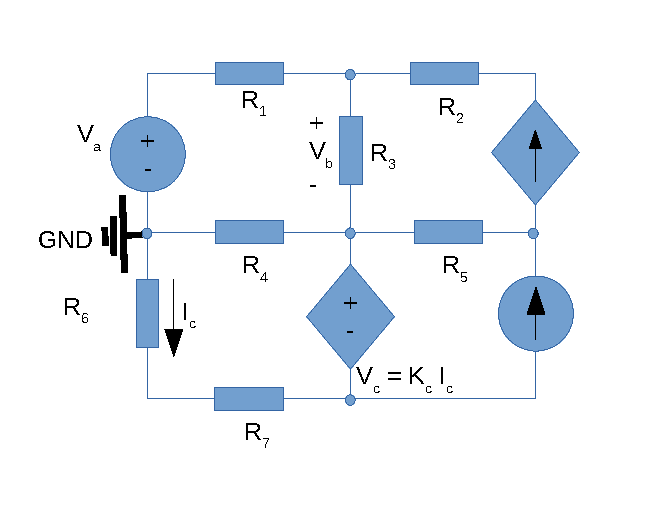
\includegraphics[width=0.6\linewidth]{circ.pdf}
	\caption{Used Circuit.}
	\label{fig:circuit}
\end{figure}





